% vim: ft=tex
\chapter{Project monitoring}
Checklist items on GitHub issues are estimated to take up to 4 hours of effort to complete.

\section{Weekly overview}

\autoref{fig:projmon:weekly} illustrates the weekly time spent on this bachelor
thesis. The thick horizontal line represents the planned effort of 28.5 hours a
week, which has been calculated using the risk analysis explained
in~\autoref{sec:projplan:est-time}.  Milestones are denoted by the green
labels. The legend along the x-axis represents the semester weeks, including
the particular RUP phases.


\begin{figure}[]
	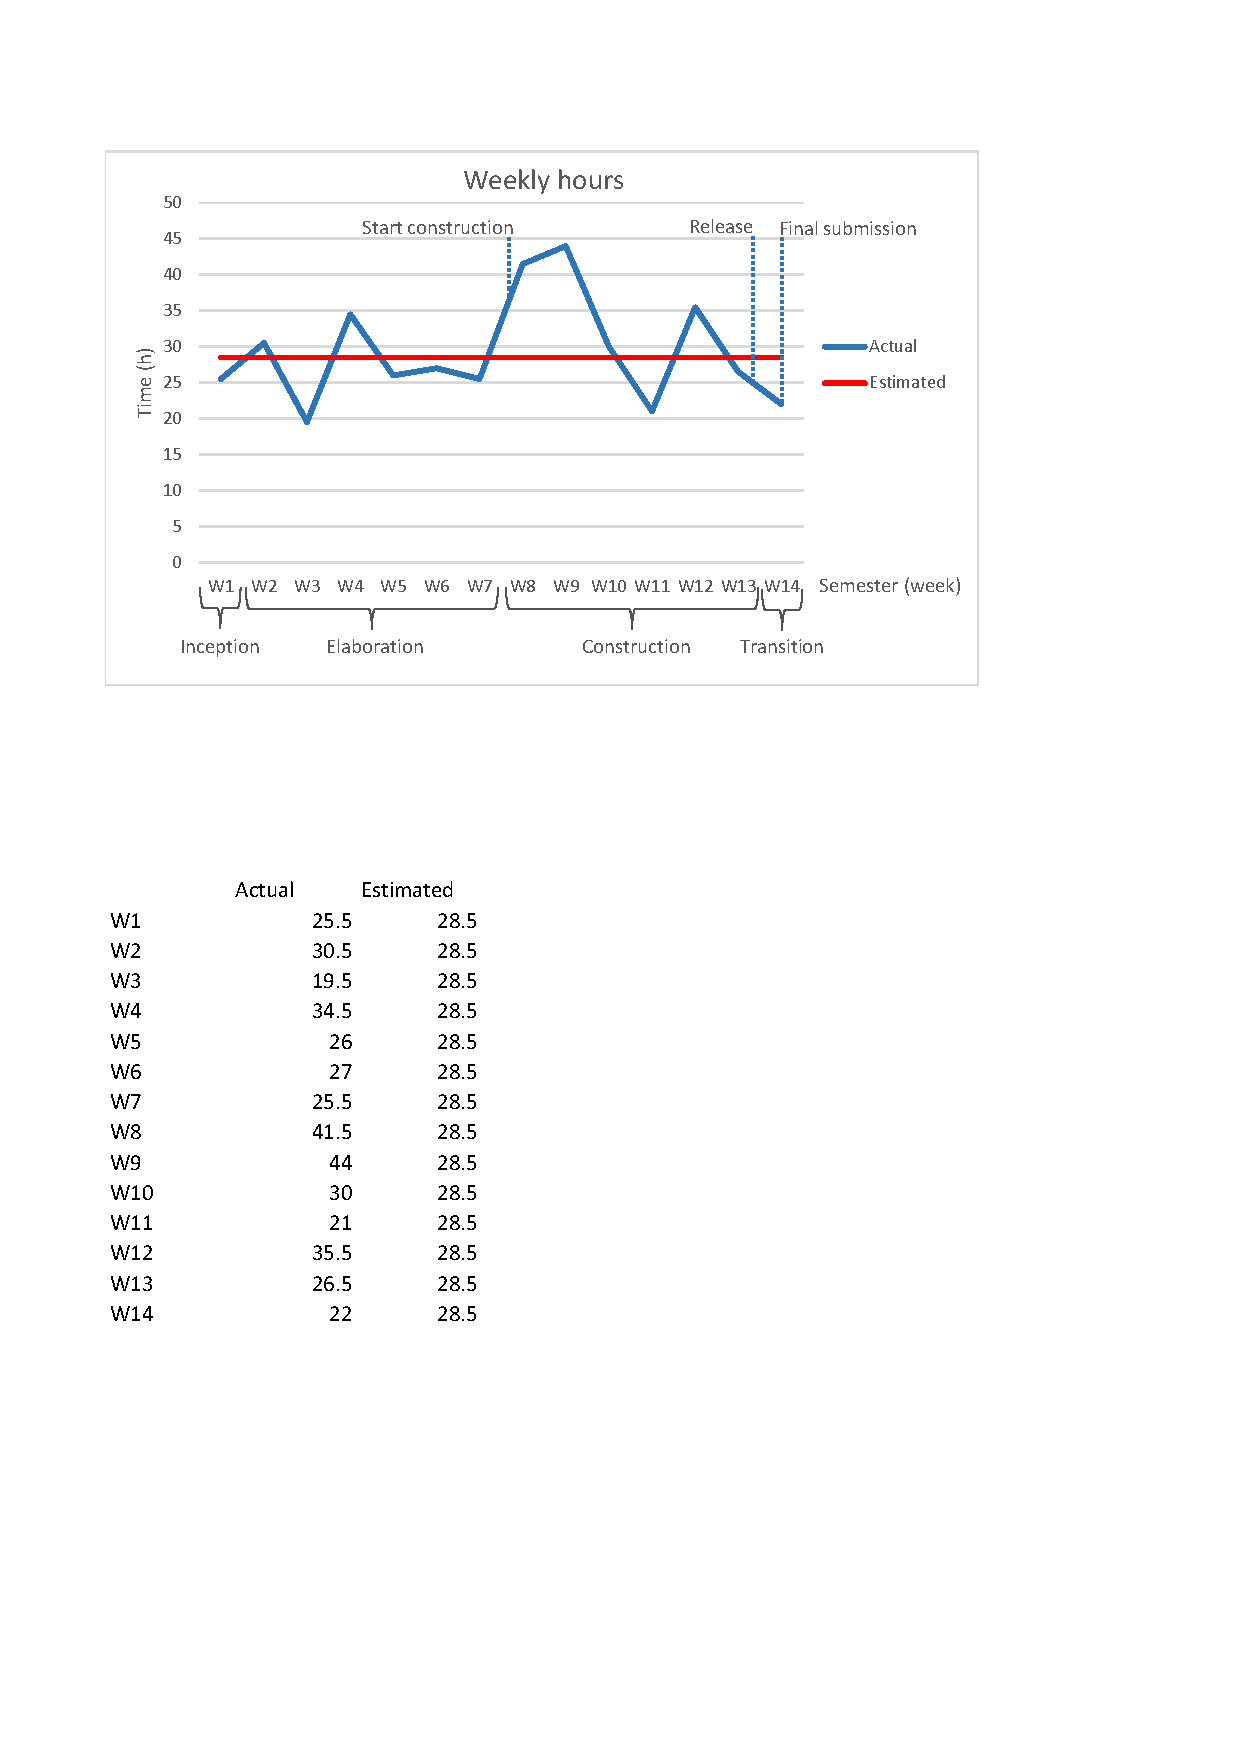
\includegraphics[trim=2cm 18.3cm 4.6cm 2.8cm, clip=true, width=\textwidth]{img/project_monitoring_weekly_hours_diagram.pdf}
	\caption{Weekly hours}
	\label{fig:weekly:hours}
\end{figure}

\begin{figure}[]
	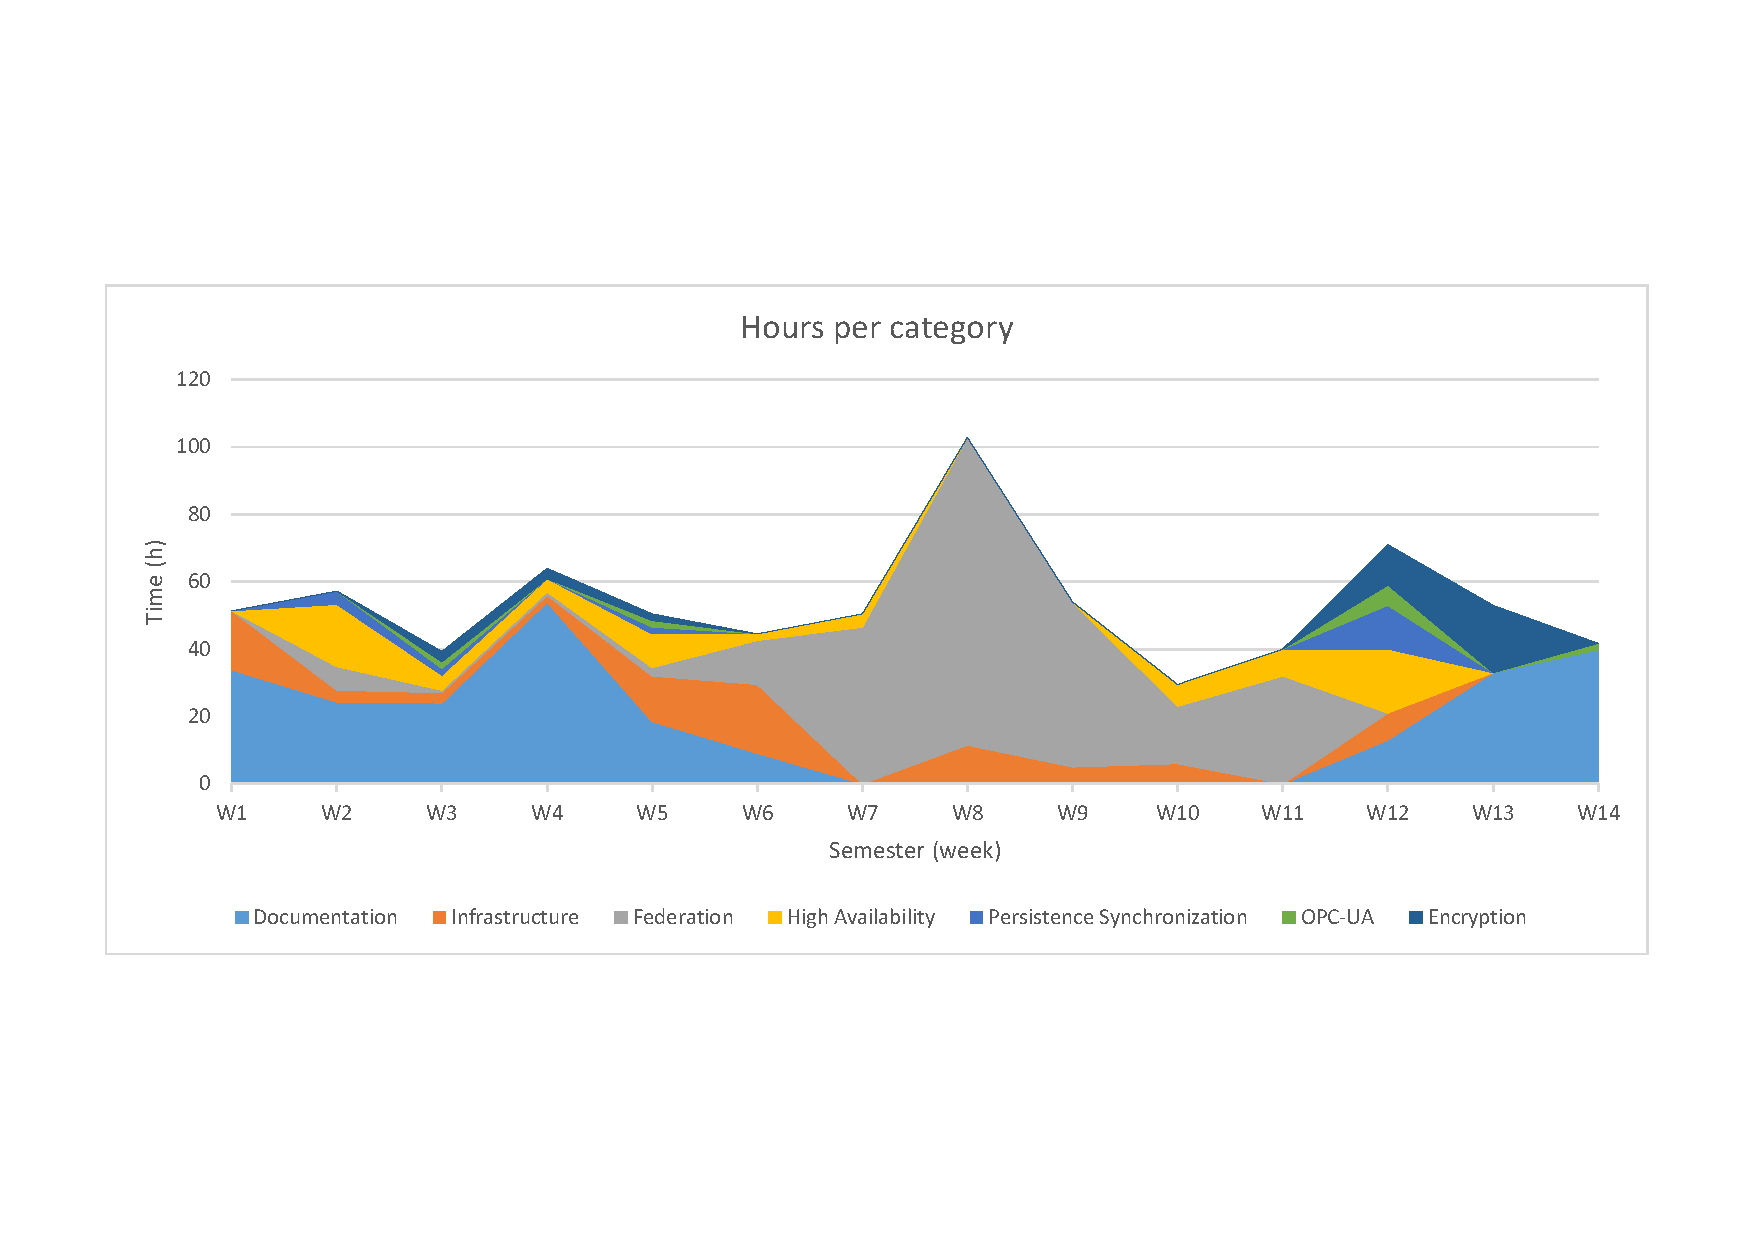
\includegraphics[trim=2cm 5cm 2cm 5.9cm, clip=true, width=\textwidth]{img/project_monitoring_weekly_hours_per_category.pdf}
	\caption{Hours per category}
	\label{fig:hours:per:category}
\end{figure}

As can be seen in the figure \autoref{fig:weekly:hours}, we have spent the
least amount of time per week at the beginning of this thesis. This is because
gathering requirements was delayed for a few days. Before the Elaboration
phase, we had all necessary information such as requirements gathered and were
ready to start with planning and the conceptual work.


\begin{table}[H]
  \centering
  \begin{tabular}{|p{100mm}|p{35mm}|}
    \hline 	\bf Planned HSR hours & 720h \\ \hline
	\bf Estimated hours & 816h \\ \hline
	\bf P. Wenger worked hours & 413h \\ \hline
	\bf M. Schuler worked hours & 403h \\ \hline
	\bf Everhour tags & 14 \\ \hline
	\bf Github issues & 94 \\ \hline
	\bf Github tasks & 230 \\ \hline
	\bf Biggest issue \#33 Refine Document & 80h \\ \hline
  \end{tabular} \\
  \caption{Project statistics}
  \label{tab:projectstats}
\end{table}


The nominal hours required by the course description have exceeded by 10\%.
The federation prototype took longer than planned. After getting more familiar with Roadster, we were able to better estimate time efforts.
\autoref{fig:hours:per:feature} illustrates the estimated versus the actual effort.

The students have a balanced hours total, because efforts and tasks were
re-evaluated on GitHub and Everhour at regular intervals.


\begin{figure}[]
	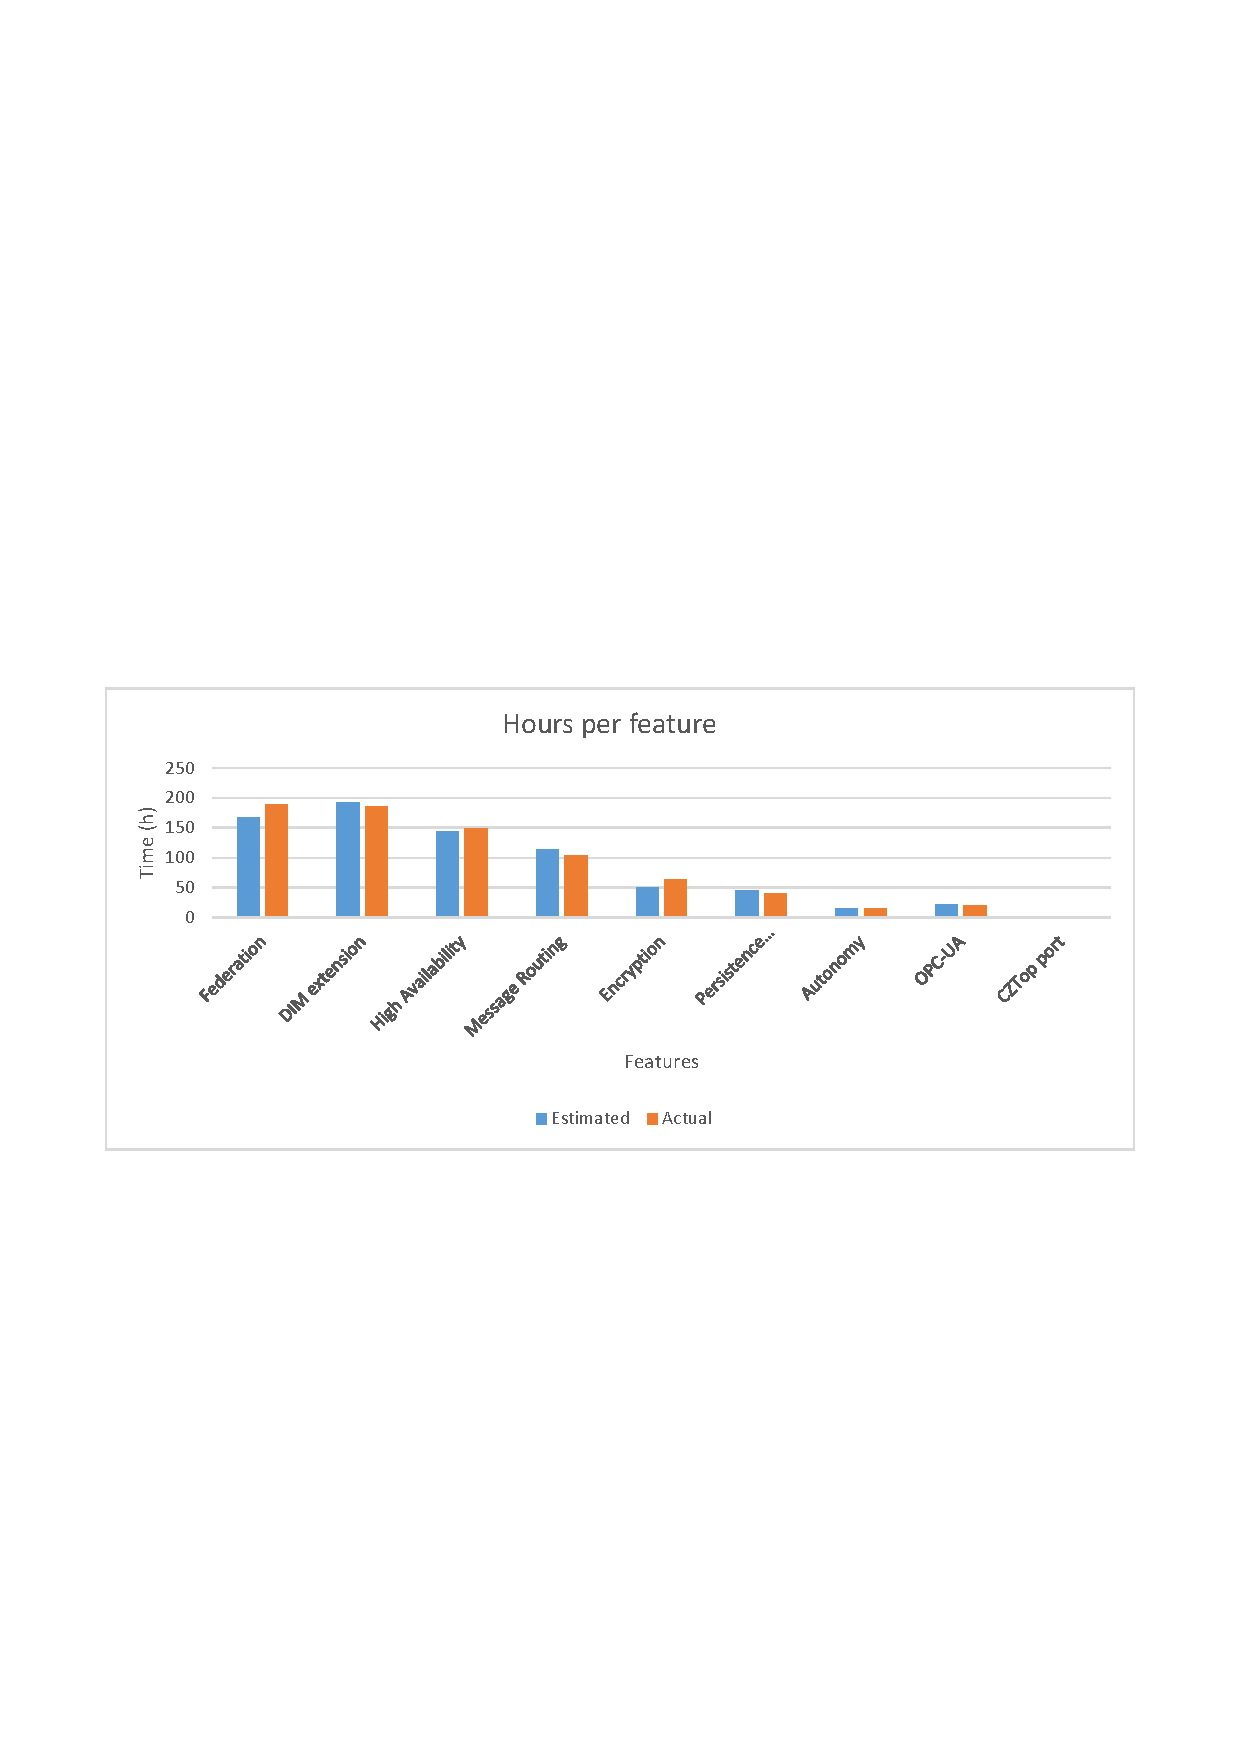
\includegraphics[trim=2cm 10.5cm 2cm 11.9cm, clip=true, width=\textwidth]{img/project_monitoring_hours_per_feature_diagram.pdf}
	\caption{Hours per feature}
	\label{fig:hours:per:feature}
\end{figure}

The exported Everhour data can be found in our final submission on Moodle. Everything can be derived from this data.

8\% of the whole project duration was used for project management and meetings. 2\% were used for requirement meetings with the client.
The distribution corresponds fully to the planned phases as shown in \autoref{fig:hours:per:tag}.
\begin{figure}[]
	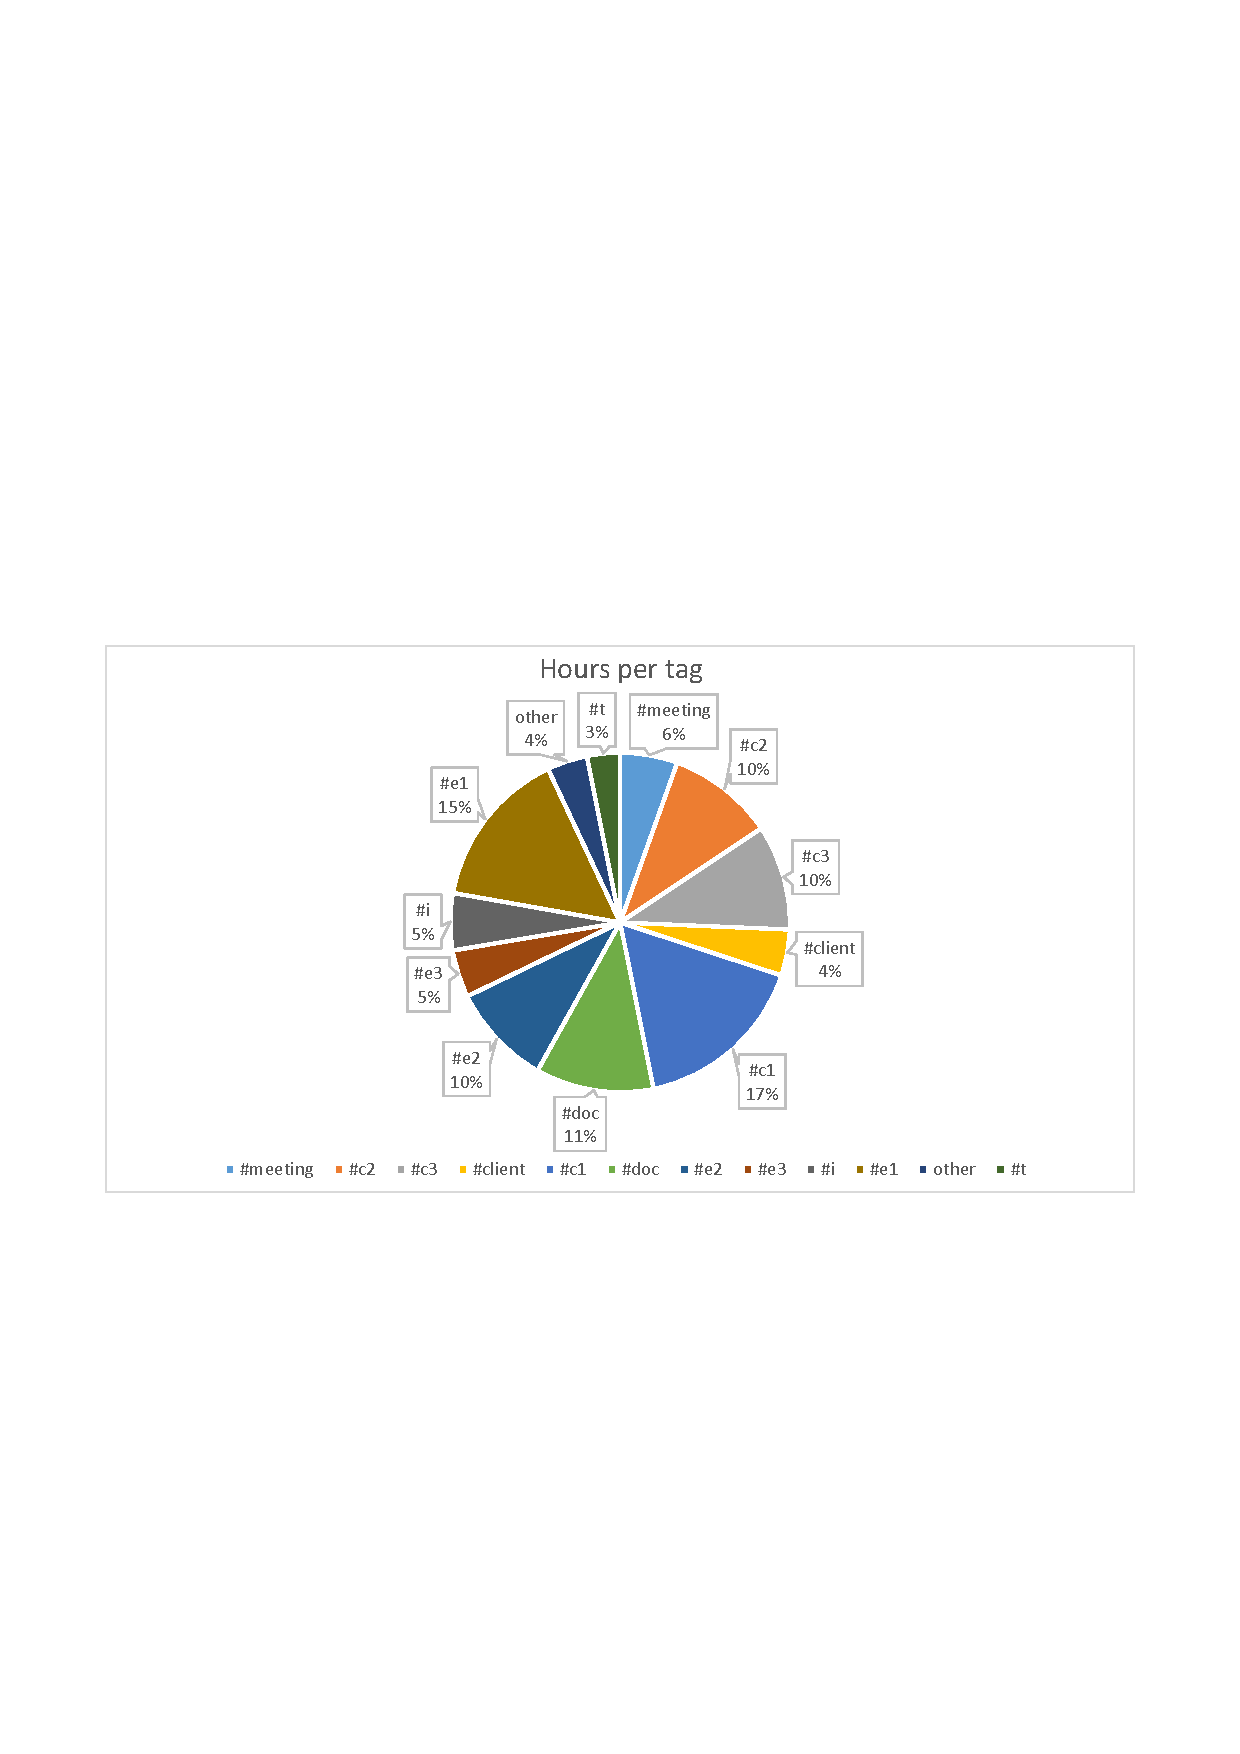
\includegraphics[trim=4cm 9.6cm 3.5cm 11.1cm, clip=true, width=\textwidth]{img/project_monitoring_hours_per_tag_diagram.pdf}
	\caption{Hours per tag}
	\label{fig:hours:per:tag}
\end{figure}

